% Rebuild: pdflatex -interaction=nonstopmode -halt-on-error obsidian.tex (three passes)
% Self-contained article. No external figures, fonts, or bibliography files required.
\documentclass[11pt,a4paper]{article}
\usepackage[T1]{fontenc}
\usepackage[utf8]{inputenc}
\usepackage{lmodern}
\usepackage[margin=25mm,headheight=15pt]{geometry}
\usepackage{microtype}
\usepackage{amsmath,amssymb,amsthm,mathtools}
\usepackage{stmaryrd}
\usepackage{booktabs,tabularx,longtable,array}
\usepackage{xcolor}
\usepackage{enumitem}
\usepackage{listings}
\usepackage{fancyhdr}
\usepackage{titlesec}
\usepackage{needspace}
\usepackage{xurl}
\usepackage[most]{tcolorbox}
\usepackage{tikz}
\usetikzlibrary{arrows.meta,positioning}
\usepackage[colorlinks=true,linkcolor=blue!35!black,citecolor=blue!35!black,urlcolor=blue!35!black]{hyperref}
\usepackage{bookmark}
\definecolor{ink}{HTML}{183044}
\definecolor{muted}{HTML}{566570}
\definecolor{accent}{HTML}{176D75}
\definecolor{pale}{HTML}{F1F5F6}
\definecolor{linegray}{HTML}{C8D4D9}
\hypersetup{pdftitle={Obsidian: Property-Aware Types and Lawful Mathematical Reasoning over Lean},pdfauthor={OpenAI, prepared for Vladimir Reshetnikov},pdfsubject={Third-round proof-language proposal, September 2026},bookmarksnumbered=true,bookmarksdepth=2}
\titleformat{\section}{\Large\sffamily\bfseries\color{ink}}{\thesection}{.6em}{}
\titleformat{\subsection}{\large\sffamily\bfseries\color{ink}}{\thesubsection}{.6em}{}
\titleformat{\subsubsection}{\normalsize\sffamily\bfseries}{\thesubsubsection}{.6em}{}
\titlespacing*{\section}{0pt}{2.8ex plus 1ex}{1.2ex}
\titlespacing*{\subsection}{0pt}{2ex plus .6ex}{.8ex}
\setlength{\parindent}{0pt}
\setlength{\parskip}{.45em}
\setlength{\emergencystretch}{3em}
\setcounter{tocdepth}{1}
\setlist{nosep,leftmargin=1.6em}
\renewcommand{\arraystretch}{1.14}
\pagestyle{fancy}\fancyhf{}
\fancyhead[L]{\small\sffamily\color{muted}OBSIDIAN / PROPERTY-AWARE MATHEMATICS}
\fancyhead[R]{\small\sffamily\color{muted}ROUND THREE}
\fancyfoot[C]{\small\thepage}
\renewcommand{\headrulewidth}{.3pt}
\newcolumntype{Y}{>{\raggedright\arraybackslash}X}
\newcolumntype{P}[1]{>{\raggedright\arraybackslash}p{#1}}
\newcommand{\code}[1]{\texttt{\detokenize{#1}}}
\newcommand{\N}{\mathbb N}\newcommand{\Z}{\mathbb Z}
\newcommand{\Q}{\mathbb Q}\newcommand{\R}{\mathbb R}
\newcommand{\Spec}{\operatorname{Spec}}
\newcommand{\den}[1]{\llbracket #1\rrbracket}
\newcommand{\EqOn}{\operatorname{EqOn}}
\newcommand{\RefineType}{\operatorname{Ref}}
\newcommand{\Jet}{\operatorname{Jet}}
\newcommand{\Lone}{\operatorname{L^1Series}}
\newtcolorbox{claimbox}[1][]{colback=pale,colframe=linegray,boxrule=.5pt,arc=1mm,left=8pt,right=8pt,top=7pt,bottom=7pt,breakable,#1}
\lstdefinestyle{obsidian}{basicstyle=\small\ttfamily,columns=fullflexible,keepspaces=true,breaklines=true,showstringspaces=false,backgroundcolor=\color{pale},frame=single,rulecolor=\color{linegray},framerule=.35pt,framesep=6pt,xleftmargin=6pt,xrightmargin=6pt,aboveskip=.8em,belowskip=.8em,tabsize=2}
\lstset{style=obsidian}
\theoremstyle{plain}\newtheorem{proposition}{Proposition}[section]
\newtheorem{theorem}[proposition]{Theorem}
\newtheorem{lemma}[proposition]{Lemma}
\theoremstyle{definition}\newtheorem{definition}[proposition]{Definition}
\theoremstyle{remark}\newtheorem{remark}[proposition]{Remark}
\makeatletter
\renewcommand*\l@section[2]{\@dottedtocline{1}{0em}{2em}{#1}{#2}}
\makeatother
\pretocmd{\section}{\Needspace{7\baselineskip}}{}{}
\pretocmd{\subsection}{\Needspace{5\baselineskip}}{}{}
\begin{document}
\begin{titlepage}
\vspace*{5mm}
{\sffamily\small\color{accent}PROOF-LANGUAGE DESIGN \quad / \quad THIRD ITERATION\par}
\vspace{12mm}
{\sffamily\bfseries\color{ink}\fontsize{40}{44}\selectfont Obsidian\par}
\vspace{5mm}
{\sffamily\bfseries\color{ink}\fontsize{25}{31}\selectfont Property-Aware Types and\\Lawful Mathematical Reasoning\\over Lean\par}
\vspace{9mm}
{\sffamily\Large A language of mathematical objects, proved properties,\\and explicitly justified changes of meaning\par}
\vspace{11mm}
\begin{claimbox}
\textbf{The central proposal.} Let the author write the mathematical structure of an argument. Let a property-aware elaborator carry the routine consequences of that structure. Every operation must still justify why the information available about its inputs is sufficient for the conclusion it produces. Properties are proved refinements of existing objects; computational observations are relations to those objects; normalization may construct a different object and must say so. Compile all three into ordinary Lean definitions and proofs before considering changes to Lean's kernel.
\end{claimbox}
\vfill
{\sffamily Prepared for Vladimir Reshetnikov\par}
{\sffamily OpenAI \quad | \quad 6 September 2026\par}
\vspace{5mm}
{\small\color{muted}Evidence status. Both specified round-two syntheses were read in full. Selected ProveIt, Fermat, and current Leant sources were inspected. This package contains a design, mathematical arguments, and 608 executed Python design probes. It is not an implemented proof language, a Lean-verified checker, or an audit of either mathematical repository. No Lean compiler was available in this environment.\par}
\end{titlepage}

\begin{abstract}
Lean already expresses mathematical properties and program behavior through dependent types, propositions, subtypes, and structures. The remaining problem is not simply missing logical expressiveness. It is that authors repeatedly reconstruct the connection between a mathematical object, its known properties, the representation currently in use, and the hypotheses that license the next operation. This article proposes \emph{Obsidian}, a conservative extension of the author-facing typing and elaboration discipline. It combines proof-backed refinement overlays, theorem-backed relational signatures for operations, and explicit contracts for constructions that change witnesses. Its intended unit is not a more powerful unstructured tactic but a mathematical step whose prerequisites, resulting information, and object identity are checked together.

The proposal builds on, rather than renames, the second round's agreement on relation-specific computation, fixed requests, scoped guards, and retained evidence. It develops two additional source cases: exact integer division in the construction of a Frey curve, and absolute-integrability contracts in a Mellin-transform proof. These expose two useful design requirements: proof obligations should often be stated under weaker, independently satisfiable interfaces than the surrounding contradiction context; and an operation must distinguish pointwise, neighborhood, almost-everywhere, and finite-order information. Current Leant source is also examined beyond the earlier summaries: its specialized Length handoff already preserves exact candidate provenance, but does not by itself provide a general Lean behavioral theorem. The article specifies a small elaboration calculus, gives a denotational soundness argument for an integer-polynomial certificate format, compares conservative and kernel-level type-system extensions, and proposes a controlled evaluation against Lean equipped with the same libraries and services.
\end{abstract}

\begingroup\small\setlength{\parskip}{0pt}\tableofcontents\endgroup
\clearpage

\section{The problem after two rounds}
\subsection{The next increment should be a typing discipline, not another grammar}
The two round-two syntheses reach a useful stopping point. Their common computational boundary is a result \(y\) accompanied by a proof of a specified relation \(R(x,y)\), checked at the original object and local context. They also agree that a witness is not a complete answer, a finite jet is not an infinite identity, and a successful external computation is not self-authenticating evidence. Those conclusions should be treated as requirements, not presented as discoveries of a third-round proposal \cite{synA,synB}.

What remains underdeveloped is the connection between this boundary and \emph{ordinary mathematical typing}. A mathematician does not repeatedly re-establish that an even integer has an even power, that a function has the regularity already proved for it, or that a locally valid identity may be differentiated on an open set. Yet a formal system must know precisely which such conclusion is justified, and precisely where it is justified. Merely adding an increasingly broad \code{obvious} tactic postpones the specification problem.

The proposed increment is therefore a language in which familiar phrases such as ``a positive real,'' ``an integrable family,'' ``the same function near this point,'' and ``a primitive solution with the same exponent'' generate \emph{different, checkable types of request}. Their evidence is available automatically when the next step needs it. The system should explain the mathematical prerequisite when that evidence is missing, rather than exposing an arbitrary implementation subgoal first.

\begin{claimbox}
\textbf{Design thesis.} Conciseness should come from reusing proved mathematical interfaces and inferring their routine consequences, not from weakening what is checked or obscuring what is claimed. Extend the \emph{surface typing judgment}; retain Lean's existing logic as the initial checking language.
\end{claimbox}

\subsection{What was actually inspected}
Both requested TeX syntheses were read completely, including their corrections, questions, and validation appendices. Their comparison of the nine proposals is used for attribution; this article does not claim an independent full reading of all nine individual reports. Fresh code inspection concentrated on the following units, rather than another broad lexical count.

\begin{center}\small
\begin{tabularx}{\textwidth}{@{}P{.25\textwidth}Y@{}}
\toprule
Inspected source & Reason for selecting it\\
\midrule
ProveIt: \path{AutonomousIteratedDeriv.lean} & A control already discussed in round two: the induction must retain a statement on an open set, not merely at one point.\\
ProveIt: \path{MellinBose.lean} & An additional worked case: termwise integration requires summability of integral norms, plus integrability and a correctly identified sum.\\
Fermat: \path{Def_FLTPrelim_FreyPackage.lean} & A mathematical structure already bundles many properties; this is evidence against claiming that Lean cannot represent such properties.\\
Fermat: \path{S_FreyPackage_of_counterexample.lean} & Successive witness changes preserve an equation while adding coprimality, parity, and a residue convention.\\
Fermat: \path{S_FreyPackage_freyCurveInt_map.lean} & Identically printed division in \(\Z\) and \(\Q\) needs a divisibility bridge.\\
Leant: verification, engine, Length handoff, and internal documentation & Candidate acceptance, exact-origin correspondence, behavioral abstraction, and kernel evidence must remain separate.\\
\bottomrule
\end{tabularx}
\end{center}

These are source-level observations, not fresh builds of those projects. The Fermat roadmap was consulted to understand the chosen files, not to certify its global proof route \cite{fltpath}. Appendix~\ref{app:sources} records paths and revisions. The new ProveIt example is not developed as a worked case in either synthesis; it is now development material, not a held-out evaluation task.

\subsection{The distinction that matters in the user interface}
Four questions should never collapse into one:
\begin{enumerate}
\item What is the object or program, with which carrier types and structures?
\item Which propositions about that exact object have been proved?
\item What relation does a new representation or result bear to it?
\item Which implementation, execution, and publication policies were used to obtain and validate the evidence?
\end{enumerate}
The first three are mathematical. The fourth includes operational metadata and trust assumptions. A proof of \(G\to Q\) may be fully checked while \(G\) remains unproved at the caller. An exact integer computation may be irrelevant to a request about rational division. A function may satisfy a length contract without satisfying a permutation contract. No single ``verified'' label adequately answers all four questions.

\section{What is inherited, and what Obsidian adds}\label{sec:delta}
\subsection{Requirements adopted from the syntheses}
Obsidian adopts fixed statement meaning before proof discovery, ordered dependent obligations, exact-target validation, theorem-backed methods, relation-specific computation, source-bound evidence, and search-independent replay. It also adopts the corrected versions of the bridge rules: complete solution sets require both soundness and coverage; neighborhood equality requires agreement on a neighborhood, not point equality plus openness; collapsed bounds can prove equality. These are important corrections to interface specifications, not merely arithmetic corner cases \cite{synA,synB}.

The proposal also accepts the reports' warning about attribution. Locus already describes bounded guard closure; Concord already propagates precision demands; Facet already proposes contract-directed representation planning; Noema already forbids cyclic guards; Meridian already develops guarded partial expressions; and Vantage already separates exact presentations, observations, and directed abstractions. Obsidian is not the first proposal to use any of these ingredients \cite{synA,synB}.

\subsection{The proposed increment}
The contribution is a particular integration and a more discriminating experiment:

\textbf{Property overlays at ordinary use sites.} Proven properties of a term become available without repeatedly wrapping and unwrapping it or registering every proposition as a type-class instance. A proof-backed overlay enriches the local context; it does not silently replace the carrier type.

\textbf{Lawful-use signatures for operations.} An operator declares, through an ordinary theorem, the input properties and relations it requires and the output relation it provides. This makes the relation discipline active \emph{inside expression elaboration}, not just at the final CAS receipt. Differentiation, integration, coefficient extraction, scalar extension, and witness normalization each obtain distinct signatures.

\textbf{Witness-changing steps are not views of the same value.} A normalized integer triple is generally not equal to the original triple. Its relation to the original, and the invariants it preserves, belong in the construction contract. This is a useful third category beside refining an unchanged object and observing an unchanged object.

\textbf{Support-restricted mathematical interfaces.} Routine bridge theorems should often expose a small set of sufficient hypotheses that can be tested outside an inconsistent proof-by-contradiction context. This is especially important for the Frey example: the high-level package is intentionally assumed for a contradiction, while the divisibility lemma itself has abundant ordinary instances.

\textbf{Behavioral synthesis with explicit semantic reach.} A structural synthesizer can search for a function of the right carrier type; additional contracts constrain which of those functions are acceptable. Specialized abstraction contracts, such as Leant's Length pipeline, should be integrated without pretending they prove arbitrary behavior of the original program.

\textbf{A matched baseline that already knows about properties.} The comparison must include existing Lean property automation and program-verification support. In particular, \code{fun_prop} already proves registered function properties compositionally, and \code{mvcgen} already generates obligations from Hoare specifications \cite{funprop,mvcgen}. The language must improve the combined authoring experience, not take credit for these capabilities.

\subsection{A criterion for useful compression}
A shorter proof is useful only when it preserves three things: the theorem's meaning, the mathematical reason offered to the reader, and a manageable path for repairing the proof after a change. A ten-line frontend proof backed by a new thousand-line one-off adapter is not automatically an improvement. Conversely, a reusable adapter may be worthwhile even when its first application costs more than an ordinary Lean proof. Both initial and amortized costs must be recorded.

\section{The author-facing language}\label{sec:surface}
\subsection{A small vocabulary}
The following listings are proposed syntax, not accepted Lean or an implemented parser. Mathematical notation would be supported in an editor; ASCII is used here to keep the source examples readily reproducible.

\Needspace{17\baselineskip}
\begin{lstlisting}
let a : Real where positive
let U : Set Real where open
let f : Real -> Real where differentiable on U

have f is continuous on U
  by differentiability

observe J of F to order 12
  by a residual certificate

construct T' from T
  preserving exponent and the defining equation
  ensuring primitive
  by gcd normalization
\end{lstlisting}

The first declaration elaborates to \(a:\R\) and a proof obligation or assumption \(0<a\), depending on whether this is an input binder or a newly defined value. The declaration of \(f\) means \(\operatorname{DifferentiableOn}\ \R\ f\ U\), not global differentiability. The observation does not replace \(F\) by \(J\). The construction names a new witness and a relation to the old one. These distinctions survive in both the expanded Lean and the compact document view.

An assumption binder may introduce a premise. A computed value declaration must prove its refinement. The same word \code{where} must not hide that difference: the editor marks an input condition as a hypothesis and a constructor condition as an obligation. An unfinished constructor does not become a theorem with an extra implicit assumption.

\subsection{Claims, reasons, and delegated details}
A mathematical claim with a named reason is checked through the named method contract. The line
\Needspace{5\baselineskip}
\begin{lstlisting}
exchange the sum and the integral
  by absolute integrability of the family
\end{lstlisting}
is not permission to prove the final equality by an unrelated theorem and retain this explanation. It asks for the hypotheses of the absolute-integrability interchange theorem. An author can instead write \code{search for a proof}, allowing discovery to select a different method, whose accepted explanation is then displayed.

Routine steps may be omitted when their goals arise from a fixed contract. Substantive choices remain authored or delegated by a fixed specification: which induction variable, which domain, which branch, which normalized object, and which kind of answer. A useful rule is that automation may fill an \emph{evidence hole} freely, while a \emph{data hole} has an explicit output specification and ownership. No provider may fill a meaning-bearing hole in a frozen theorem header.

\subsection{Progressive disclosure without semantic concealment}
The compact view shows the mathematical claim and its reason. A second view exposes the generated obligations, such as \(4\mid n\), summability of norms, or the membership \(x\in U\). A third view shows the exact Lean theorem applications and proof terms. The first view must still show restrictions that change the claim: a domain, a root branch, finite precision, conditionality, or completeness. This implements the syntheses' visibility rule rather than replacing it with a style preference \cite{synA}.

A failed exact-division step should therefore report:
\begin{claimbox}
The requested integer-to-rational transport needs \(16\mid -a^p b^p\). Evenness of \(b\) supplies a factor \(2^p\), but the current context has not established \(4\le p\). The expression still has an integer quotient; equality with the rational quotient has not been proved.
\end{claimbox}
This is more informative than either a generic type mismatch or a silent fallback to rational arithmetic. A reader need not inspect the particular \code{Rat.intCast_div} application to understand what is missing.

\section{A conservative property-aware type system}\label{sec:types}
\subsection{Lean already has the underlying expressiveness}
Lean's subtype \(\{x:A\mid P(x)\}\) contains a value and a proof. Subtypes are already used for mathematical and programming invariants; proof fields do not require an additional run-time representation. Ordinary dependent functions can express postconditions, and structures can bundle algebraic data with laws \cite{subtypes}. The Frey package is an immediate source-level example \cite{freydef}.

Thus the proposal is not ``add predicates to a language that lacks them.'' It is to organize how predicates participate in elaboration. There are three distinct representations of known properties:
\begin{center}\small
\begin{tabularx}{\textwidth}{@{}P{.24\textwidth}Y Y@{}}
\toprule
Form & Best use & Cost to control\\
\midrule
Unbundled value and proofs & Local mathematics and incremental discovery & Evidence must remain associated with the exact value and scope.\\
Subtype or proof-carrying record & Exported interfaces and returning certified data & Repeated repackaging and coercion paths can obscure the unchanged carrier.\\
Type class or bundled structure & Coherent reusable operations and structural laws & Instance selection can change data or meaning; arbitrary facts should not become global instance search.\\
\bottomrule
\end{tabularx}
\end{center}
Obsidian uses the first form internally for most local refinement, the second at chosen boundaries, and the third where Lean already expects an algebraic structure. It does not replace all three with a universal ``property type.''

\subsection{Carrier typing and refinement typing}
Let \(\Gamma\) be an ordered Lean context with fixed universes, constants, and instance choices. Write
\[
 \Gamma\vdash e\rightsquigarrow t:A
\]
for elaboration of a surface expression to a Lean term. A refinement judgment adds proof evidence:
\[
 \Gamma\vdash t:A\mid\Phi
 \qquad\text{with}\qquad
 \Phi=(p_1:P_1(t),\ldots,p_k:P_k(t)).
\]
The notation does not change \(t\)'s Lean type. It records ordinary propositions with ordinary checked inhabitants. Predicates may mention other objects and parameters: \(\operatorname{Coprime}(a,b)\), \(\operatorname{Integrable}(f,\mu)\), and \(f=g\) on \(U\) are not forced into a unary vocabulary at the logical level.

At a public boundary, the same content can be compiled as
\[
 \RefineType(A,P)=\{x:A\mid P(x)\},
 \qquad
 \RefineType(A,P\wedge Q)=\{x:A\mid P(x)\wedge Q(x)\}.
\]
Intersection here means multiple properties of \emph{one carrier value}. It does not identify \(\{x\mid P(x)\}\) and \(\{x\mid Q(x)\}\) as Lean types. Proof irrelevance does not make arbitrary predicates definitionally equal.

\subsection{Core elaboration rules}
The following rules describe proof construction, not a new oracle for deciding truth.

\textbf{Refine.} From \(t:A\) and \(p:P(t)\), register the fact \(P(t)\) for that term. No new value is created.

\textbf{Forget or project.} A requested subset of the known propositions can be supplied by projecting the evidence. Forgetting a refinement never licenses a change of carrier or interpretation.

\textbf{Entailment.} If a registered theorem, instantiated in \(\Gamma\), has type
\[
 h:\forall x:A,\ P(x)\to Q(x),
\]
then \(p:P(t)\) yields \(h\ t\ p:Q(t)\). More general rules have an ordered dependent telescope of premises. Registration checks the theorem's actual type, not an unchecked signature string.

\textbf{Contract application.} If
\[
 h:\forall x:A,\ P(x)\to R(x,f(x)),
\]
a request to apply \(f\) with guarantee \(R\) generates \(P(t)\), supplies its proof, and returns \(f(t)\) together with \(h\ t\ p\). The requirement can be discharged by local facts, structural property propagation, a bounded solver, or an explicit subproof.

\textbf{Dependent construction.} A method may return
\[
 \prod_{x:A}\prod_{h:P(x)}\ \sum_{y:B(x,h)} R(x,h,y).
\]
The witness is bound after its prerequisites. It cannot be moved outside those binders by treating the obligations as an unordered set. In the simpler case where \(B\) and \(R\) do not depend on \(h\), the interface can hide the proof argument; this simplification is justified by the actual types, not by typography.

\textbf{Transport.} A change from a value or representation \(x\) to \(y\) uses a theorem with a specified relation. Equality supports ordinary substitution. A weaker relation supports only registered respectful operations, developed in Section~\ref{sec:relations}.

\subsection{Bidirectionality and bounded search}
The carrier type and resolved operators are inferred first, or checked against an expected type. Expected refinements then generate obligations. Some facts are propagated forward from constructors and hypotheses; other obligations are requested backward by the next method. This combination avoids trying to enumerate every true property of every local object.

The default search is intentionally incomplete. It uses direct facts, registered projection and structural rules, a bounded transition depth, and named solver profiles. Repeated requests share already checked evidence. A failed route means ``this obligation was not discharged,'' not ``the property is false.'' Arbitrary predicate implication contains general theorem proving; adding it to a typing interface does not make it decidable.

Current \code{fun_prop} is an especially important precedent and implementation component. It composes registered function-property theorems, uses local hypotheses, and limits transitions between properties to control search growth \cite{funprop}. Obsidian should reuse this machinery where it fits. Its proposed addition is that the inferred property is integrated with source obligations, relational use sites, and retained evidence, rather than requiring every author to call a separate tactic at each such boundary.

\subsection{Proof properties versus mathematical structure}
``Commutative ring'' usually contains operations as well as laws. ``The chosen element is a unit'' is a proposition about a value in that structure. These must not be conflated. If two ring structures on the same carrier have different multiplication, a proof about one cannot discharge a goal about the other because both render as multiplication.

Accordingly, algebraic operations, topology, measure, scalar actions, and meaningful coercions are part of the frozen carrier context. Proposition-level evidence may be inferred relative to that context. The elaborator must not upgrade a ring to a field to satisfy a CAS request, or use classical choice to supply executable data without an explicit noncomputable interpretation. Competing data-bearing instances require deterministic selection or a visible ambiguity; proof irrelevance is not a cure for structural incoherence.

\subsection{Scopes, support, and branch joins}\label{sec:support}
Each retained fact has a checked proof term and its dependency support. Support includes free variables in the proof, their types, and the transitive local declarations required to type those variables. It also records global theorem dependencies for policy and replay. It is not an asserted mathematically minimal set of hypotheses.

Evidence may move to another context only through a checked context embedding or an explicitly abstracted theorem. At the end of a block, a fact mentioning a local witness must remain local, be packaged with that witness, or be abstracted over it. Renaming the witness does not remove the dependency. A fact established under \(x\ne0\) in one case cannot become available in its sibling case through a cache key containing only the printed goal.

A branch join is an ordinary logical elimination: when the cases cover the original context and each branch proves the same postcondition, the postcondition can be retained outside. If the case split uses excluded middle, that dependency is recorded. A list of branch labels is not a coverage proof.

Guard assembly is a directed proof graph. A node may depend only on evidence already justified in its permitted context. Using a proposed result to establish its own prerequisite is rejected. This does not ban mathematical induction or recursive definitions: their cycles are governed by a separate induction or termination theorem, not by arbitrary back-edges in the obligation graph.

\subsection{What the basic soundness claim actually says}
\begin{proposition}[Relative elaboration soundness]\label{prop:elab}
Fix a Lean environment and a well-typed statement context. Suppose every registered logical rule is backed by a theorem in that environment, every accepted application supplies terms of the theorem's actual premise types, and every generated obligation is discharged. Then the core rules above construct Lean evidence for their recorded conclusions in the translated context. A completed assertion has no residual guard assumptions except those present in its declared statement.
\end{proposition}
\begin{proof}
Induct on the finite elaboration derivation. Refinement retains the supplied proof. Projection uses an existing proof or conjunction elimination. Entailment and contract application instantiate a theorem and apply it to proofs supplied by the induction hypotheses. Dependent construction uses its theorem's dependent pair and eliminator without changing binder order. Transport uses the registered transport theorem. Scope exit abstracts over the retained dependencies or packages them; a branch join uses the checked eliminator and coverage evidence. Each operation is an ordinary Lean term former, so its type is the advertised conclusion in the translated context.
\end{proof}

This is a paper argument about the specified core, not a machine-checked compiler-correctness theorem. Rechecking emitted terms still matters. More importantly, term validity does not establish that a compromised parser or renderer represented the author's intended statement. The source-to-statement interpretation and the exported challenge statement remain separate validation surfaces, as Lean's own validation guidance emphasizes \cite{validation}.

\section{Lawful-use signatures: properties meet relations}\label{sec:relations}
\subsection{An operator needs the right kind of information}
A unary property describes one object. Many dangerous proof shortcuts concern two objects and an operation: may one function replace another before differentiating, integrating, or extracting a coefficient? The relevant contract has the schematic form
\[
 C(\vec x,\vec y)\ \land\ \bigwedge_i R_i(x_i,y_i)
 \quad\Longrightarrow\quad
 S\bigl(F(\vec x),G(\vec y)\bigr).
\]
All the \(R_i\), \(S\), operators, and side conditions are ordinary Lean expressions. A registry entry adds search indices and human-readable roles to a theorem of this form. It does not add a new logical rule.

The central elaboration question becomes: \emph{does the available information justify this use of the result?} Equality has an extensive collection of substitution principles. A finite jet, enclosure, or almost-everywhere identity has a smaller and differently shaped collection. The system propagates the consumer's requirements through the appropriate theorem rather than first choosing a convenient representation and hoping it is adequate.

\begin{center}\small
\begin{tabularx}{\textwidth}{@{}P{.22\textwidth}P{.35\textwidth}Y@{}}
\toprule
Operation & Sufficient information in a typical contract & Information that is not enough\\
\midrule
Evaluate at \(x\) & Equality at \(x\) & Almost-everywhere equality with no information about \(x\).\\
Differentiate at \(x\) & Equality in a neighborhood of \(x\); derivative-existence evidence when the conclusion asserts existence & Equality only at \(x\).\\
Replace under an integral & Almost-everywhere equality for the same measure; the chosen analytic theorem's integrability premises & Equality for a different measure or an arbitrary sampled set.\\
Extract coefficient \(k\) & A jet certified below \(N\), with \(k<N\) & A jet whose cutoff is at most \(k\).\\
Cast an integer quotient to \(\Q\) & Exact divisibility and a nonzero denominator & A merely nonzero denominator.\\
Normalize a solution & A construction preserving the specified equation and parameters & Equality of the new tuple with the old one, which is generally false.\\
\bottomrule
\end{tabularx}
\end{center}

The hypotheses in this table are illustrative sufficient contracts, not claims of universal weakest preconditions. Some totalized Lean operators admit equalities even when their usual analytic interpretation is unavailable. An author requesting differentiability or a convergent integral must receive the stronger specification, not just an equality between totalized values.

\subsection{Locality is part of the relation}
Let \(U\subseteq\R\) be open and \(x\in U\). From \(\EqOn(f,g,U)\) one obtains eventual equality at \(x\), because \(U\) is a neighborhood of \(x\). A derivative-transfer theorem can use that eventual equality. The input proposition carries \(U\), the point \(x\), and membership evidence; none is incidental metadata.

Almost-everywhere equality is different. For Lebesgue measure, changing a function at one point preserves its almost-everywhere class but can change its value at that point. Replacing an integrand may therefore be legitimate while replacing its point evaluation is not. A ``function equality'' label without its filter or measure is too weak an interface.

The same principle handles representation maps. Forward preservation of a polynomial identity under a ring homomorphism is different from reflection of an equality through an injective map. Neither implies unrestricted reflection of existential properties, such as ideal membership after extending integer coefficients to rationals. These distinctions are inherited from the syntheses; the new mechanism is to make each operation ask for the appropriate relation during elaboration \cite{synA,synB}.

\subsection{Precision is a dependent input, not a confidence score}
For formal power series over a commutative ring, write
\[
 A\equiv_N B\quad\Longleftrightarrow\quad
 [t^k]A=[t^k]B\quad\text{for every }k<N.
\]
Addition and multiplication preserve the minimum of the input cutoffs. Differentiation sends agreement below \(N+1\) to agreement below \(N\). Extracting \([t^k]A'\) consequently demands input agreement through coefficient \(k+1\), namely a cutoff of at least \(k+2\). Each arithmetic condition is itself an obligation with checked evidence.

These contracts are sufficient, not always optimal. In positive characteristic, differentiation can lose less information on special inputs. A factor known to have high valuation can improve a product's required precision. Such improvements belong in additional theorems, not a global heuristic that changes the meaning of ``order.'' A cached higher-precision observation can answer a lower-precision query by a proved restriction map; the reverse direction requires new information.

\subsection{Demand planning and its limits}
A planner may propose a route from the available relations to the desired one. The route checker validates each theorem application, its guards, its intermediate objects, and its final specification. This separates a potentially expensive, heuristic planning problem from a small proof reconstruction problem. It also gives a concrete failure report: the requested derivative coefficient needs one more input coefficient, rather than an unexplained failure of a normalization tactic.

Initially, routes should be shallow and stable. Automatic domain shrinking is forbidden when the request names a larger domain. Changing a branch or constructing a new witness is not an invisible route optimization. A different exact polynomial normalizer may be substituted without notice when it returns the same requested guarantee and satisfies the same trust policy. This distinction follows the mathematical observation, not merely whether the serialized answer changed.

\section{Case study: Frey parameters and exact division}\label{sec:frey}
\subsection{The source already uses property-carrying objects}
The inspected \code{FreyPackage} contains nonzero integers \(a,b,c\), a natural exponent \(p\), primality and \(5\le p\), the equation \(a^p+b^p=c^p\), a coprimality condition, and the congruences \(a\equiv3\pmod4\), \(b\equiv0\pmod2\). Derived lemmas supply oddness of \(p\), further coprimality facts, and nonvanishing products. This is a successful use of Lean's existing structures, not evidence that the type system cannot express mathematical invariants \cite{freydef}.

Nevertheless, the integer and rational Weierstrass models are defined separately. Their nontrivial coefficients have the same printed form:
\[
 a_2=\frac{b^p-1-a^p}{4},\qquad
 a_4=\frac{-a^p b^p}{16}.
\]
In the integer model, division is integer division. In the rational model, it is field division. The source proof that the integer model maps to the rational model explicitly establishes divisibility before using the cast-of-division theorem. It then handles the remaining coefficients by straightforward extensionality \cite{freymap}.

This is exactly the kind of detail a mathematician compresses as ``the model is integral.'' It is also exactly the detail a language must not erase. Nonzero denominators alone do not make integer division exact: \(\lfloor5/2\rfloor=2\), whereas \(5/2\in\Q\) is not \(2\).

\subsection{Extract a weaker arithmetic interface}
The proof of coefficient integrality uses much less than an entire Frey package. Define
\[
 \operatorname{Admissible}(a,b,p)\quad\Longleftrightarrow\quad
 p\text{ is odd},\quad 4\le p,\quad
 a\equiv3\pmod4,\quad 2\mid b.
\]
Here \(a,b\in\Z\) and \(p\in\N\). Oddness and \(4\le p\) imply \(5\le p\), but primality, nonvanishing, coprimality, and the Fermat equation are not needed. There are many actual instances, including \((a,b,p)=(3,2,5)\).

\begin{proposition}[Exact Frey coefficients]\label{prop:frey}
If \(\operatorname{Admissible}(a,b,p)\), then
\[
 4\mid b^p-1-a^p,
 \qquad
 16\mid -a^p b^p.
\]
Consequently, the corresponding integer quotients, embedded into \(\Q\), equal the displayed rational quotients.
\end{proposition}
\begin{proof}
Write \(b=2k\). Since \(p\ge4\), both \(4\mid b^p\) and \(16\mid b^p\). The congruence \(a\equiv3\equiv-1\pmod4\) and oddness of \(p\) imply \(a^p\equiv-1\pmod4\), hence \(4\mid1+a^p\). Subtracting gives the first divisibility; multiplying \(16\mid b^p\) by \(-a^p\) gives the second.

For the last assertion, if \(n=dk\) with \(d\ne0\), exact integer division gives \(n/d=k\). In \(\Q\), applying the integer embedding to \(n=dk\) and cancelling the nonzero image of \(d\) gives the same quotient \(k\). Apply this with \(d=4\) and \(d=16\).
\end{proof}

The value \((3,2,5)\) gives the integer coefficients
\[
 a_2=(32-1-243)/4=-53,
 \qquad a_4=-243\cdot32/16=-486.
\]
No counterexample to Fermat's theorem is involved in this arithmetic test.

\subsection{A proposed definition interface}
A definition package could express the coefficients once, with their exactness obligations attached to the integer construction:
\Needspace{16\baselineskip}
\begin{lstlisting}
def integralModel(a, b : Int; p : Nat)
    requires Admissible(a, b, p)
    : WeierstrassCurve Int :=
  coefficients
    a1 = 1
    a2 = exact_quotient (b^p - 1 - a^p) by 4
    a3 = 0
    a4 = exact_quotient (-a^p * b^p) by 16
    a6 = 0

have map_to_rationals(integralModel(a,b,p))
       = rationalModel(a,b,p)
  by coefficientwise exact-division transport
\end{lstlisting}

\code{exact_quotient} does not redefine ordinary integer division. It is a constructor whose result includes a proof that multiplication by the denominator recovers the numerator, and whose chosen implementation can use integer division. The package proves the connection between this constructor, ordinary division, and rational embedding. A caller that merely requests integer division receives no exactness property automatically.

The frontend expands the final method into coefficient equality, the two divisibility lemmas, cast transport, and routine algebra. An ordinary Lean wrapper can provide exactly the same proof. The proposed language's added value is making the obligations predictable and making the mathematical phrase ``integral coefficients'' available as a reusable interface, not inventing a new theorem prover.

\subsection{Negative neighbors reveal distinct missing hypotheses}
Dropping different premises fails in different ways:
\begin{center}\small
\begin{tabularx}{\textwidth}{@{}P{.27\textwidth}P{.22\textwidth}Y@{}}
\toprule
Dropped requirement & Parameters & Failure\\
\midrule
Odd exponent & \((3,2,4)\) & \(b^p-1-a^p=-66\), not divisible by \(4\).\\
Residue of \(a\) & \((1,2,5)\) & The numerator of \(a_2\) is \(30\), not divisible by \(4\).\\
Evenness of \(b\) & \((3,3,5)\) & The numerator of \(a_2\) is \(-1\).\\
Exponent lower bound & \((3,2,3)\) & The numerator of \(a_4\) is \(-216\), not divisible by \(16\).\\
\bottomrule
\end{tabularx}
\end{center}
In the last row, the rational quotient is \(-27/2\), whereas the integer quotient by positive \(16\) is \(-14\). The system should identify the exact bridge that failed; rejecting every cast would also reject the legitimate positive cases and would not constitute a useful safety mechanism.

\subsection{A subtle test-design problem: vacuous local contexts}\label{sec:vacuity}
A full Frey package is introduced as part of a proof by contradiction. Once a theorem of the form \(\operatorname{FreyPackage}\to\mathrm{False}\) is available, every proposition follows in that context, including a badly specified arithmetic bridge. This is not a flaw in Lean: elimination of falsehood is valid. It is a flaw in a test that interprets arbitrary success under an impossible premise as evidence that the arithmetic interface is correctly specified.

The remedy is not a general consistency checker. It is to test reusable arithmetic contracts under independently meaningful premises, such as \(\operatorname{Admissible}\), and to exhibit concrete satisfying inputs. A method intended to justify exact division should use its arithmetic premises and theorem dependencies, not a downstream global contradiction. The support-restricted interface in Section~\ref{sec:support} makes this visible and enforceable as a \emph{method policy}.

This policy is stronger than axiom auditing in one respect and weaker in another. A perfectly valid theorem with only standard logical axioms can still prove a local claim vacuously. Conversely, forbidding a particular contradiction theorem does not prove that all remaining premises are consistent. The language should therefore report the actual support and use satisfiable contract tests, while making no claim to solve general consistency or automatically discover weakest hypotheses.

The same issue applies outside number theory: impossible dimensional constraints, empty subtypes, and contradictory branch conditions can make a behavioral specification vacuous. A good test suite records a positive inhabitant where feasible, not merely that a proof compiles.

\subsection{Normalization is a succession of new witnesses}
The inspected normalization proof first divides out a common factor, then arranges that the second coordinate is even, then chooses a sign so that the first coordinate is \(3\pmod4\). Its existential tuples repeatedly carry the equation and the newly established invariants. The parity stage may swap coordinates or replace a triple by \((a,-c,-b)\); the sign stage may negate all three coordinates. Oddness of the exponent is essential to the sign arguments \cite{freynorm}.

A concise account should represent this as a sequence of contracted constructions:
\Needspace{17\baselineskip}
\begin{lstlisting}
assume T is a nonzero counterexample at exponent p
have p is odd
  by primality and p >= 5

construct T1 from T, primitive
  preserving exponent and equation
  by division by the common gcd
construct T2 from T1, with second coordinate even
  preserving exponent, equation, and primitivity
  by the parity alternatives
construct T3 from T2, with first coordinate = 3 mod 4
  preserving exponent, equation, primitivity, and parity
  by simultaneous sign choice
return the Frey package carried by T3
\end{lstlisting}

This is not a six-line proof for free. Each construction needs an ordinary theorem, and its cost belongs in the implementation accounting. The language gains a stable interface for the recurring preservation facts. It must not record \(T=T_1=T_2=T_3\); those equalities are generally false. Scaling, permutation, and sign relations are construction provenance, not equality of representations of a fixed tuple.

There is a further specification issue in the inspected source: the exported conclusion is \code{Nonempty FreyPackage}, not a package indexed by the input exponent. The proof body preserves \(p\), but the conclusion alone does not expose that fact \cite{freynorm}. A proposed interface returning a package \(P\) with \(P.p=p\) is therefore a stronger contract that needs its own proof. Obsidian must not infer such an exported guarantee merely because the body appears to preserve the parameter.

\section{Case study: an absolutely integrable Mellin family}\label{sec:mellin}
\subsection{The mathematical argument and its formal interfaces}
For \(a>0\), the inspected ProveIt module proves
\begin{equation}\label{eq:mellin}
 \int_0^\infty x^{a-1}\log(1-e^{-x})\,dx
 =-\Gamma(a)\zeta(a+1).
\end{equation}
Its final Lean theorem expresses the real zeta value through the real part of the complex Riemann zeta function. The development establishes the logarithmic series, integrability of rescaled Gamma kernels, the integral and integral norm of each summand, summability of those norms, and then applies an interchange theorem \cite{mellin}.

The essential family is
\[
 F_n(x)=-\frac{x^{a-1}e^{-(n+1)x}}{n+1},\qquad n\in\N,
 \qquad \mu=\text{Lebesgue measure restricted to }(0,\infty).
\]
For every \(x>0\), the logarithmic series gives
\[
 \sum_{n=0}^\infty F_n(x)=x^{a-1}\log(1-e^{-x}).
\]
Positive rescaling of the Gamma integral gives
\begin{align*}
 \int F_n\,d\mu&=-\frac{\Gamma(a)}{(n+1)^{a+1}},\\
 \int |F_n|\,d\mu&=\frac{\Gamma(a)}{(n+1)^{a+1}}.
\end{align*}
The second equality uses the nonpositivity of \(F_n\) on the domain. Since \(a+1>1\), the series of integral norms converges. That is the substantive justification for exchanging sum and integral; the rest is identification of the resulting scalar series.

\subsection{A behavioral refinement for a family}
For real-valued functions on a measure space, define
\[
 \Lone(\mu,F):=
 \bigl(\forall n,\ \operatorname{Integrable}(F_n,\mu)\bigr)
 \ \land\
 \operatorname{Summable}\!\left(n\mapsto\int |F_n|\,d\mu\right).
\]
This is a property of an entire family, not a pointwise property of one term. It has a straightforward Lean definition using \code{Integrable} and \code{Summable}. A theorem-backed operator can consume it to obtain the interchange equality. Identification of the pointwise sum with a particular function is another premise, usually supplied on the domain or almost everywhere.

There is no need for a new primitive type named ``absolutely integrable family.'' An alias, an ordinary predicate, and a package of introduction and elimination theorems suffice logically. The author-facing type system makes that package usable as a refinement:
\Needspace{18\baselineskip}
\begin{lstlisting}
let a : Real where positive
let mu = volume restricted to (0, infinity)
let F[n](x) = -x^(a-1) * exp(-(n+1)*x) / (n+1)

have each F[n] is integrable for mu
  by the positively rescaled Gamma kernel
have integral_mu |F[n]| = Gamma(a)/(n+1)^(a+1)
  by the Gamma integral and the sign of F[n]
have F is an L1-summable family for mu
  by the p-series criterion, since a+1 > 1

have sum_n F[n](x) = x^(a-1)*log(1-exp(-x)) on x>0
  by the logarithmic series
conclude the Mellin identity
  by exchange of sum and integral, then the zeta series
\end{lstlisting}

The positivity of \(n+1\), cast normalization, and compatibility of real and complex powers on positive arguments are routine obligations generated by these methods. They should be inferred and retained, not restated at every use. The nontrivial fact that the integral norms form a convergent \(p\)-series should remain visible. The refined type therefore helps distinguish an analytic idea from the routine algebra needed to use it.

\subsection{Why pointwise convergence is not the relevant type}
A sharp negative test is available on \((0,1)\) with Lebesgue measure. For \(n\ge1\), let
\[
 f_n(x)=n\,\mathbf1_{(0,1/n)}(x).
\]
Every \(f_n\) is integrable with integral \(1\), but \(f_n(x)\to0\) for every \(x>0\). Thus pointwise convergence and termwise integrability do not justify interchanging a limit and an integral.

For an actual \emph{series} counterexample, put
\[
 g_0=f_1,\qquad g_n=f_{n+1}-f_n\quad(n\ge1).
\]
The partial sums telescope to \(f_{N+1}\). Therefore \(\sum_{n\ge0}g_n(x)=0\) for every \(x\in(0,1)\), whereas
\[
 \sum_{n\ge0}\int g_n\,dx=1,
 \qquad
 \int\sum_{n\ge0}g_n\,dx=0.
\]
For \(n\ge1\), the difference is \(1\) on \((0,1/(n+1))\) and \(-n\) on \((1/(n+1),1/n)\), up to irrelevant endpoints. Hence
\[
 \int|g_n|\,dx=\frac1{n+1}
 +n\left(\frac1n-\frac1{n+1}\right)=\frac2{n+1}.
\]
The required series of integral norms diverges. This negative neighbor is stronger than merely omitting a line from the Mellin proof: it shows that the weaker proposed contract would be mathematically false even though every individual term is integrable and the pointwise sum exists.

\subsection{Total operators and analytic intent}
A Lean expression for an integral or an infinite sum is still a well-typed expression when hypotheses needed for a familiar analytic interpretation are missing. A property-aware frontend must not infer integrability from the existence of that expression. Nor should it globally replace Lean's total operators by partial ones, thereby changing the meaning of existing source.

The default for imported Lean code is its existing semantics. A new mathematical document may select a lexical convention in which a ``convergent integral'' request includes an integrability contract, or an exact quotient includes divisibility. Such conventions are visible and elaborated explicitly. Ordinary total-value equality and convergence-certified equality remain different specifications.

\section{A control case: induction, locality, and finite observations}\label{sec:analysis}
\subsection{The autonomous derivative theorem}
The ProveIt control theorem assumes \(U\) open and \(W'=\varphi\circ W\) on \(U\). It takes families \(G_n\) and \(G'_n\) with the required differentiability and recurrence only at points in the range \(W(U)\), then proves
\[
 D^nW(x)=G_n(W(x))\qquad(n\in\N,\ x\in U).
\]
The source induction first retains the whole statement on \(U\), uses openness to obtain equality near the chosen point, and only then differentiates and applies the chain rule. Its more convenient globally differentiable corollary is explicitly separate \cite{autonomous}.

The correct surface plan is therefore:
\Needspace{10\baselineskip}
\begin{lstlisting}
prove for all n: D^n W = G[n] composed with W on U
  by induction on n, retaining the whole domain U
  base: use the zeroth-order identity
  step:
    differentiate the induction identity locally on U
    use the chain rule and W' = phi composed with W
    use the recurrence for G at values attained by W
\end{lstlisting}

``Retaining the whole domain'' is mathematically meaningful: it fixes the induction motive. If the induction hypothesis were only an equality at one fixed point, the derivative step would not follow. The elaborator may suggest the uniform motive, but accepting a stronger motive is an explicit proof-plan decision, not a silent strengthening of the theorem's assumptions.

Range-local differentiability is another important refinement. Demanding global differentiability of every \(G_n\) can exclude valid applications with poles outside \(W(U)\). The method should generate exactly the local hypotheses in its theorem, rather than normalize all requests to a stronger and easier-to-find global property.

\subsection{Residual certificates remain an inherited computational service}
For a formal series \(\Delta\) defined implicitly, an observation may be obtained without constructing a preferred global solution. The general residual theorem emphasized by Locus and the syntheses has the following form \cite{synA,synB}. Let \(R\) be a commutative ring, \(F(Y)\in R[[t]][Y]\), and suppose
\[
 F(\Delta)=0,\quad \Delta(0)=d,\quad J(0)=d,
 \quad F(J)\equiv_N0,
\]
where \(N\ge1\). If the derivative of the coefficientwise reduced polynomial \(\overline F\in R[Y]\) at \(d\) is a unit, then \(J\equiv_N\Delta\).

For completeness, factor the polynomial difference as
\[
 F(J)-F(\Delta)=(J-\Delta)H.
\]
The constant coefficient of \(H\) is \(\overline F'(d)\); thus \(H\) is a unit of \(R[[t]]\). Since the left side is divisible by \(t^N\), so is \(J-\Delta\). This proves the observation relation for the \emph{already given} \(\Delta\). It proves neither existence of \(\Delta\) nor a full infinite identity from one finite computation.

Obsidian's addition is to connect this service to lawful use: a demand for \([t^k]\Delta'\) requests sufficient residual precision and then uses the derivative observation theorem. The candidate \(J\) remains a finite observation of the original object. Its coefficient data is not silently substituted into the theorem's quantifier over \(\Delta\).

The inherited negative examples remain essential. Over \(\Z/4\Z\), \(F(Y)=2Y\), \(\Delta=0\), and \(J=2t\) have zero residual but do not agree below order \(2\); a nonzero derivative is not enough. For \(F(Y)=Y^2-1\), choosing \(J=-1\) cannot certify the jet of the selected root \(\Delta=1\) merely because both are roots. The branch condition is part of the specification.

\section{Behavioral constraints and Leant}\label{sec:leant}
\subsection{A function type is not the whole synthesis target}
A request for \(f:A\to B\) permits every function of that type. A behavioral request instead fixes a proposition about the function, for example
\[
 \sum_{f:A\to B}\ \forall x:A,\ P(x)\to Q(x,f(x)).
\]
When \(P\) and \(Q\) encode length, sortedness, equation preservation, or analytic behavior, they genuinely restrict the acceptable outputs. They also create additional proof work. A rich type does not make that work disappear; it makes the work impossible to overlook.

For example, preserving list length does not imply preserving elements, preserving their order, or sorting them. A sorting request needs at least an order specification and a permutation specification, with the relevant order structure fixed. A normalization request on integer triples needs its equation and parameter-preservation laws, not simply a function returning a triple with coprime first two entries. Behavioral contracts must be selected to match the user's actual objective.

For mathematical objects, a first implementation should usually synthesize an unbundled candidate and a separate theorem about it, then package both at acceptance. This allows ordinary theorem search to manipulate the proof obligation while structural synthesis chooses the candidate. It avoids forcing the search engine to understand every dependent type construct before it can be useful.

\subsection{Current source adds a specialized behavioral boundary}
The current \code{Verification.hs} explicitly describes \code{Verified} as an opaque receipt of callback acceptance, not a kernel proof or behavioral certificate. The generic verification pass tries rendered variants under a quota, and its accepted-spelling filter preserves the accepted occurrence rather than manufacturing authority for skipped duplicates \cite{leantverify}.

The inspected engine and internal documentation also retain richer candidate provenance than a bare rendered string: an exact typed candidate, its run authority, provider bindings, and a renderer origin. The specialized \code{Length.Handoff} takes a \code{Verified DetailedVerificationVariant}, checks source/search correspondence and exact rendering, resolves the configured family and provider laws, and prepares a candidate-specific Djex Length problem. Its own comment carefully limits the claim to structural correspondence for that adapter \cite{leantengine,leanthandoff,leantdocs}.

This is important context for round three. It would be inaccurate to describe the current tree as having no behavioral-contract machinery. It would be equally inaccurate to promote its correspondence receipt into a general theorem of Lean about the candidate. The retrieved head is the same revision identified in the earlier reports; the point is additional inspection of a boundary not developed in their shared summaries, not a claim that a new commit appeared during this review.

\subsection{The adapter Obsidian should implement}
A Obsidian request contains the exact Lean carrier target, behavioral proposition, permitted local telescope, selected structures, and origin identity. The provider receives only the intended search interface. Candidate acceptance should proceed through the following distinct judgments:
\begin{center}\small
\begin{tabularx}{\textwidth}{@{}P{.24\textwidth}Y@{}}
\toprule
Judgment & Meaning\\
\midrule
Carrier accepted & The exact candidate elaborates at the requested Lean type.\\
Correspondence accepted & The analyzed candidate and the displayed or committed candidate are bound to the same origin and rendering.\\
Abstract contract established & A specified behavioral model satisfies its requested property, by the evidence route that model provides.\\
Original contract proved & A Lean proof establishes the behavioral proposition about the original candidate, including any adequacy or interpretation theorem required by abstraction.\\
Publication accepted & The committed source or retained proof replays, has no unresolved obligations, and satisfies the declared dependency and execution policy.\\
\bottomrule
\end{tabularx}
\end{center}

The first three do not imply the fourth without a justified bridge. Existing Leant identity preservation is valuable input to that bridge; replacing it with text-based heuristics would be a regression. The generic adapter should preserve, rather than flatten, specialized refusal reasons.

For tactic suggestions, the exact accepted edit must be replayed at the source origin before it is called a completed proof. The syntheses identify this as a separate requirement from successfully probing a tactic. This article does not report a fresh audit or repair of every current tactic-suggestion path \cite{synA,synB}.

\subsection{What structural synthesis might usefully compose}
The relevant benchmark population is not an arbitrary list of easy lemmas. The case studies generate genuine composition tasks:

In the Frey bridge, synthesis can assemble evenness into power divisibility, combine the exponent bound with divisibility monotonicity, obtain the residue of an odd power, and supply the exact-division theorem's two premises. A solver that merely retrieves the entire bridge theorem should be measured separately from one that assembles those steps.

In the Mellin package, synthesis can combine integrability of a rescaled kernel with scalar multiplication, use sign information to turn an integral norm into an ordinary integral, and assemble the two components of \(\Lone\). It should not discover the Gamma integral or the appropriate interchange principle accidentally under the guise of routine inference.

In the derivative control, the task is to combine open-domain equality, neighborhood membership, derivative transport, and the chain rule while retaining the range-local hypotheses. This is a natural structural-composition target because the mathematical plan is supplied and the remaining work consists of fitting dependent theorem interfaces together.

These obligations can be exported as a frozen benchmark with matched theorem availability, bounded resources, and a record of which successful proofs used lookup, synthesis, or arithmetic. No productivity result is claimed here.

\subsection{Negative outcomes and behavioral evidence}
A complete search in a restricted calculus may show that no term exists \emph{in that calculus}. It does not automatically prove the negation of the original Lean proposition. A counterexample in an abstract behavior model may also be spurious unless it is realizable by an original input. An abstraction bit, an empty warning list, or a solver's status string is not an adequacy theorem.

A safe protocol distinguishes unsupported input, bounded failure, complete fragment nonderivability, checked abstract counterexample, and a proof or refutation of the original specification. Only the last category can directly discharge a Lean proposition. These distinctions are required even when a specialized domain has excellent internal validation \cite{synA,synB,leantengine}.

\subsection{Behavior includes operational semantics when the claim says so}
Some Leant invariants are operational: quota checks precede forcing later list elements, rejected spellings may be retried, and accepted duplicates do not create new semantic authority. A theorem solely about the final finite list of accepted values does not prove that an implementation avoids forcing an undefined tail. For a lazy Haskell program, that claim needs a semantics of evaluation or an appropriate trace model.

For Lean programs, Hoare specifications and weakest-precondition reasoning are already supported by \code{Std.Do} and \code{mvcgen}; Dijkstra-monad work provides an established foundation for effect-indexed verification \cite{mvcgen,dijkstra}. Obsidian should offer an authoring layer over such specifications when the objects under discussion are programs. For an external Haskell service, it must additionally account for the implementation-to-model connection. An output contract is not a proof of termination, resource use, absence of side effects, or fidelity of a foreign-language runtime.

Consequently, three behavioral levels should remain separate: extensional mathematical behavior of returned functions; safety properties of a modeled execution trace; and total-correctness or cost claims relative to a stated operational semantics. A cost bound in an abstract model is not a wall-clock guarantee.

\section{A small certified algebra service, specified end to end}\label{sec:cas}
\subsection{Do not ask an opaque CAS to define equality}
The type discipline needs useful producers, but it does not require an unrestricted CAS. A first algebra service can normalize integer-coefficient expressions and check ideal-membership certificates. A discovery engine may be untrusted. The acceptance theorem must refer to the original mathematical expressions, not just to a Boolean result on an unrelated encoding.

The companion program contains an executable integer-polynomial checker. Its role here is to test the proposed format and adversarial inputs. It is Python, not a Lean-verified component. The mathematical interpretation and soundness argument below specify what a Lean implementation must establish; they are not evidence that such an implementation has already been built.

\subsection{Representation and denotation}
Fix a finite number \(m\) of atom slots. A sparse polynomial is a finite map
\[
 P:\N^m\longrightarrow\Z.
\]
Zero coefficients are omitted and exponent vectors have exactly \(m\) nonnegative integer entries. For a commutative ring \(R\) and a valuation \(\rho:\{0,\ldots,m-1\}\to R\), define
\[
 \den{P}_{\rho}
 =\sum_{\alpha\in\operatorname{supp}P}
   \iota(P(\alpha))\prod_{j=0}^{m-1}\rho(j)^{\alpha_j},
\]
where \(\iota:\Z\to R\) is the canonical homomorphism. This interpretation works in rings with zero divisors and in positive characteristic. It does not require an injective integer embedding.

Addition is coefficientwise addition, negation negates coefficients, and multiplication is finite convolution:
\[
 (P Q)(\gamma)=\sum_{\alpha+\beta=\gamma}P(\alpha)Q(\beta).
\]
The finite-map implementation must reject malformed dimensions and noninteger coefficients. A format explicitly designed for integer coefficients must not silently admit a rational multiplier that changes the coefficient domain.

\begin{lemma}[Denotation respects operations]\label{lem:denotation}
For the representation above,
\[
 \den{P+Q}_{\rho}=\den P_{\rho}+\den Q_{\rho},\quad
 \den{-P}_{\rho}=-\den P_{\rho},\quad
 \den{P Q}_{\rho}=\den P_{\rho}\den Q_{\rho}.
\]
\end{lemma}
\begin{proof}
Extend both finite maps by zero over the union of their supports for addition. Distributivity of finite sums and the homomorphism laws for \(\iota\) give the first two identities. For multiplication, expand the product of the two finite sums. Commutativity in \(R\) groups each product of monomials into the monomial with exponent vector \(\alpha+\beta\). Grouping the finitely many equal exponent vectors gives precisely the convolution coefficient. No reflection from functions to formal polynomials is used.
\end{proof}

A reified expression grammar needs only integer constants, indexed atoms, addition, negation, multiplication, and powers by natural \emph{literals}. Its normalizer maps these constructors to the corresponding sparse operations. Induction on the expression, using Lemma~\ref{lem:denotation} and induction for powers, proves that normalization preserves denotation. An arbitrary symbolic exponent is not a literal and must remain an atom or be handled by a separately proved symbolic theorem.

\subsection{Certificate checking and the original expression}
Given a target polynomial \(g\), equation polynomials \(f_1,\ldots,f_s\), and proposed multipliers \(q_1,\ldots,q_s\), the checker verifies
\begin{equation}\label{eq:cert}
 g-\sum_{i=1}^{s}q_i f_i=0
\end{equation}
as equality of normalized finite coefficient maps. It first checks exact list arity. A truncating zip operation on mismatched input lists is not an acceptable protocol rule.

\begin{theorem}[Soundness of the coefficient certificate]\label{thm:cert}
If the checker accepts \eqref{eq:cert}, then for every commutative ring \(R\) and valuation \(\rho\),
\[
 \bigl(\forall i,\ \den{f_i}_{\rho}=0\bigr)
 \quad\Longrightarrow\quad \den g_{\rho}=0.
\]
\end{theorem}
\begin{proof}
Interpret the accepted coefficient identity in \(R\). Lemma~\ref{lem:denotation} gives
\(\den g_{\rho}=\sum_i\den{q_i}_{\rho}\den{f_i}_{\rho}\).
Each summand is zero under the hypotheses.
\end{proof}

To close a Lean goal about expressions \(E,E_i\), the adapter also needs checked reification equalities
\[
 E=\den g_{\rho},\qquad E_i=\den{f_i}_{\rho}.
\]
The valuation is bound to the \emph{exact Lean terms} occupying the atom slots, including local-variable and instance identity. Two atoms with the same printed name are not identified by typography. These equalities, the certificate theorem, and the original hypotheses \(E_i=0\) reconstruct a proof of \(E=0\).

The atoms need not be algebraically independent: a polynomial identity valid for every valuation remains valid at a dependent valuation. The converse does not follow. Agreement at selected values does not prove coefficient equality, and a failed coefficient search does not refute the original expression.

\subsection{Execution is a separate proof obligation}
Even after a Lean theorem establishes the soundness of the checker function, a byte string returned by a compiled producer is not automatically a proved output of that function. The strict route establishes the relevant evaluation equality through kernel reduction or another checked proof, then applies the soundness theorem. A native-evaluation route uses its actual trust assumptions and is recorded separately. Source bindings and reification are required in both routes.

The second-round syntheses ran limited toolchain experiments on this distinction and on a bounded \code{grobner} tactic. Their timings do not establish general multivariate performance, and their experimental Boolean checker lacked its denotational theorem \cite{synA,synB}. Obsidian therefore makes no new performance claim from those results. Existing proof-producing tactics, including \code{ring}, \code{linear_combination}, and the configured \code{grobner} route, are controls and possible producers, not competing logical foundations.

The initial \code{grobner} adapter should record the actual toolchain, coefficient structures, resource limits, and proof evidence returned by that invocation. Successful production of a checked proof is useful; failure under its limits is not a decision of nonmembership. A reusable independent certificate-export interface must be implemented or demonstrated, not assumed because a tactic succeeds.

\subsection{What was executed in the companion}
The symbolic tests check
\[
 X^n-Y^n=(X-Y)\sum_{k=0}^{n-1}X^{n-1-k}Y^k,
 \qquad 1\le n\le32,
\]
and reject the corresponding multiplier with its constant coefficient increased by one. They also reject mismatched arities, mismatched variable spaces, noninteger coefficients, and a request lacking the commutative-ring contract. These are exact symbolic coefficient computations, not numerical sampling. Separate small evaluation tests check the implementation's arithmetic on selected integer valuations.

The companion does not parse Lean terms, generate Lean evidence, prove its own Python implementation correct, or defend against arbitrary hostile Python objects. Its supported data is built by the validated constructors in the script. A production boundary must parse and validate all serialized inputs and must impose explicit size and resource limits before normalization. The checked format and the mathematical soundness argument identify the work needed for a genuine verified core rather than obscuring it behind a success count.

\section{Should Lean's kernel type system be extended?}\label{sec:kernel}
\subsection{Four different proposals are often called a type-system extension}
The user-facing ambition deserves a direct answer. There are at least four substantially different ways to make properties feel like types:
\begin{center}\small
\begin{tabularx}{\textwidth}{@{}P{.22\textwidth}Y Y@{}}
\toprule
Option & Change & Assessment for Obsidian\\
\midrule
Library refinements & Predicates, subtypes, structures, and wrappers & Necessary first substrate; immediately interoperable with Lean.\\
Property-aware elaboration & Automatic proof arguments, local overlays, relational signatures, structured obligations & Recommended first language extension; changes how terms are written and elaborated, not accepted logic.\\
Primitive kernel refinements & A new refinement constructor and certificate-bearing subsumption rules & A possible later experiment, requiring a translation or direct metatheory and measured benefit.\\
Semantic conversion & Treat proved mathematical equivalences or CAS normalization as definitional equality & Not recommended as the initial design; substantially enlarges the conversion problem.\\
\bottomrule
\end{tabularx}
\end{center}

Calling only the last two ``real'' type-system work would miss the practical objective. An elaborator that infers the proof argument needed by a refined function application changes the author's type-directed programming model, even when the kernel receives ordinary dependent products and applications. Conversely, syntax alone without a stable inference and obligation discipline is not enough.

\subsection{Why native refinement types could still be worthwhile}
A kernel primitive might reduce coercion bureaucracy or support a more principled elaborator interface. One possible design has a constructor \(A\{P\}\), an introduction form carrying \(t:A\) and \(p:P(t)\), an erasing projection, and explicit subsumption evidence for \(P\Rightarrow Q\). A translation to Lean's current subtype and function constructs could justify conservativity if it preserves typing and the intended reduction behavior.

However, that statement is a research obligation, not an automatic consequence of the notation. Dependent occurrences, universe levels, proof irrelevance, reduction, and equality of projections must be addressed. Lovas and Pfenning's work on refinements for logical frameworks is a relevant precedent precisely because the correspondence with proof-irrelevant predicates is mathematically nontrivial \cite{lovas}. Its decidability results for its chosen system are not a license to add arbitrary mathematical entailment to Lean's conversion procedure.

Obsidian should first measure whether ordinary subtypes and unbundled proofs actually create an irreducible performance or usability cost after the elaborator is improved. If they do, a primitive refinement experiment should ship a precise translation, preservation theorems, and benchmarks against that existing implementation. Until then, the conservative version supplies a stronger basis for learning what primitive support is needed.

\subsection{Why arbitrary subsumption must not become conversion}
Consider a proposed implicit rule that accepts \(x:A\{P\}\) wherever \(A\{Q\}\) is expected exactly when \(P\Rightarrow Q\) is mathematically true. For unrestricted Lean propositions, determining whether the rule applies includes arbitrary theorem proving. It cannot be implemented as a general complete terminating inference procedure merely by calling it subtyping.

There are two disciplined alternatives. The subsumption step can require a supplied proof, whose checking is delegated to Lean. Or automatic inference can use a restricted decidable fragment with a sound translation and a failure state that does not assert falsity. Obsidian uses the first as the logical rule and the second as one optional automation mechanism.

Similarly, replacing definitional equality with unrestricted polynomial, analytic, or quotient reasoning is not merely an optimization. Even a proof-producing rewrite system used automatically in conversion needs carefully controlled reduction and congruence behavior. The initial design keeps such equivalences propositional and inserts explicit proof terms at use sites. A theorem that two computations agree is useful without turning them into the same kernel expression.

\subsection{Partiality, behavior, and effect types}
Partial mathematical operations can be represented by an explicit domain and a value on that domain. Effectful programs can be represented by a monad and a specification logic. Neither requires making mathematical undefinedness identical to program failure or making program failure identical to an unproved proposition.

A partial quotient package, for example, distinguishes the total Lean expression \(a/b\) from an operation whose domain requires \(b\ne0\). The package may also distinguish a field quotient from an exact integer quotient. Its coercions and bridges are explicit. A behavioral program type can instead quantify over input states, output states, and returned values, with an exception postcondition if needed. A partial-correctness statement need not assert termination; a total-correctness request must.

The recommended extension is consequently stratified in a literal sense: ordinary carrier types; proof-backed value and family refinements; relational observation contracts; and, where needed, effectful program specifications. There is no universal subtype ordering that collapses all these dimensions.

\section{Elaboration, evidence, and collaborative editing}\label{sec:implementation}
\subsection{A concrete pipeline}
The following pipeline is a proposed implementation architecture, not a deployed service.
\begin{center}
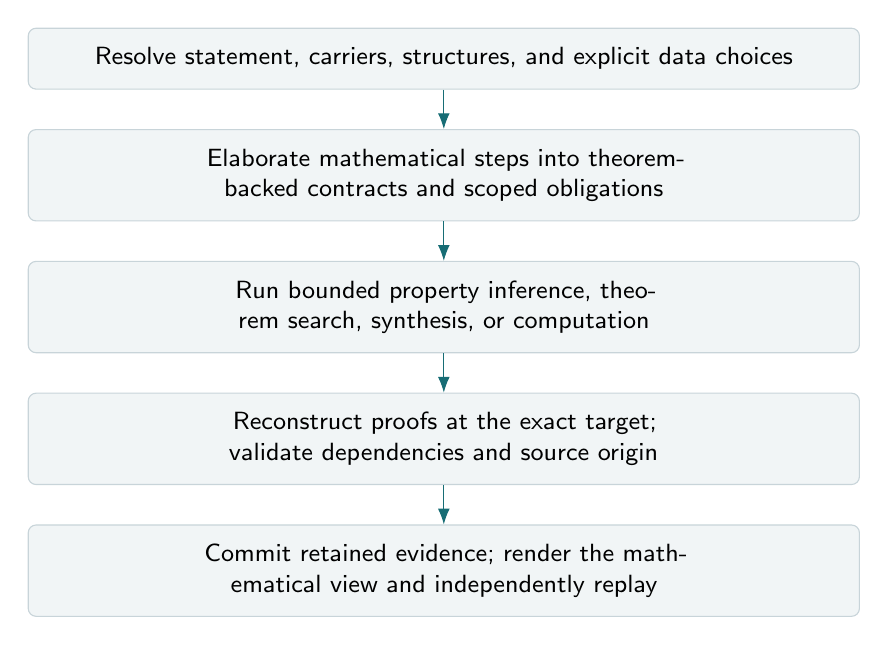
\begin{tikzpicture}[node distance=5mm, every node/.style={font=\small\sffamily}, box/.style={draw=linegray,fill=pale,rounded corners=1mm,text width=.83\textwidth,align=center,inner sep=7pt}, >={Latex[length=2mm]}]
\node[box] (s) {Resolve statement, carriers, structures, and explicit data choices};
\node[box,below=of s] (p) {Elaborate mathematical steps into theorem-backed contracts and scoped obligations};
\node[box,below=of p] (q) {Run bounded property inference, theorem search, synthesis, or computation};
\node[box,below=of q] (r) {Reconstruct proofs at the exact target; validate dependencies and source origin};
\node[box,below=of r] (v) {Commit retained evidence; render the mathematical view and independently replay};
\draw[->,color=accent] (s)--(p);\draw[->,color=accent] (p)--(q);\draw[->,color=accent] (q)--(r);\draw[->,color=accent] (r)--(v);
\end{tikzpicture}
\end{center}

The first phase resolves all choices that determine the theorem's meaning. Unresolved carrier, instance, universe, and branch choices cannot be handed to an untrusted proof provider as convenient freedoms. Explicitly delegated data construction is represented by a separate request with a fixed specification.

A method registry indexes actual Lean theorems by semantic roles: subject, domain, premise, output, precision, and explanatory reason. These roles belong to a stable project-owned wrapper, not guessed positions in an upstream theorem's telescope. When an upstream library changes, the wrapper is rechecked. A role mismatch is an adapter failure, not an opportunity to reinterpret the document.

The obligation phase reuses Lean's context and metavariable machinery. New state should record operations that Lean does not already expose conveniently: source-to-proof links, a mathematical obligation view, object-indexed observation records, and origin-sensitive validation. Duplicating Lean's entire local context in an independent workspace would create another consistency problem without a demonstrated benefit \cite{synA,synB}.

\subsection{Dependent guard composition}
Suppose a first method has type
\[
 T_1:\forall x,\ G(x)\to\sum_y R(x,y),
\]
and a second has type
\[
 T_2:\forall x\,y,\ R(x,y)\to H(x,y)\to\sum_z S(x,y,z).
\]
Given \(g:G(x)\), the first method produces \(y,r\). Only then is the second guard instantiated as \(H(x,y)\). Its proof must concern that retained \(y\), not some other output that could have been chosen. The result carries both \(R(x,y)\) and \(S(x,y,z)\), or a proved composition thereof.

A compiler may schedule independent proof tasks concurrently, but a scheduler cannot reorder semantic dependencies. Nor may it replace the intermediate witness with a different one after a downstream guard has been proved. Shared data metavariables are committed transactionally; alternative searches run against snapshots and must not partially mutate the accepted state.

\subsection{Evidence records and cache reuse}
A retained node needs an exact statement, local telescope, proof term or checked certificate, source origin, resolved constants and structures, and policy-relevant dependencies. Operational fields include producer identity, budget, and diagnostic status. Those fields help reproduce work but are not proofs.

An exact request match is a useful cache fast path. More general reuse needs an explicit adapter showing that the retained guarantee supplies the new one in the current context. This covers higher-to-lower jet precision, a larger-to-smaller domain, and a narrower-to-wider enclosure. The adapter also proves any object correspondence and supplies the current guards. A hash is an efficient identity check, not a substitute for these entailments \cite{synA}.

Evidence involving a chosen topology, measure, or scalar structure must retain that choice. Two terms printing as \code{f} are not the same request merely because their strings match. Source edits that change only proof presentation can preserve the mathematical request; edits changing definitions, quantifiers, branch selection, or data-bearing instances cannot.

\subsection{Collaboration and upgrades}
Two authors may independently prove new properties of the same unchanged object. Their proof nodes can be merged when the object, context, and environment correspond and both proofs recheck. If they independently change the chosen witness or representation route, the merge is not simply the union of their fact sets. Downstream statements must either be transported to a chosen version or remain on separate branches.

A practical merge receipt should classify changes as evidence-only, plan, object, or statement changes, following the syntheses, and identify the first affected obligation. The useful addition is a replayable witness or route correspondence, not a promise that semantic merge conflicts can be decided automatically.

A library or toolchain upgrade produces a new validation receipt. Old evidence remains historical evidence for its old environment. In particular, native-evaluation policies are interpreted against the destination toolchain's actual axiom inventory rather than an inherited blacklist of one axiom name. A dependency change may be mathematically harmless but still requires rechecking at the new interface.

\subsection{Trusted boundaries and publication}
For routine development, ordinary kernel checking protects against many mistakes in tactics and elaboration. For unreviewed agent-generated code, the proof-production process must also be isolated from the trusted statement and validation process. Lean's validation documentation distinguishes these threats and describes independent statement comparison and proof replay as stronger checks \cite{validation}.

Obsidian's publication pass checks every formal assertion in the document, even if the final theorem does not use it. It reports residual conditions, actual assumptions, and trust policy. A named reason is linked to its contract application; a prose assertion that was never formalized is marked as commentary rather than displayed with the same status as a checked lemma. The renderer must not upgrade ``conditional,'' ``finite,'' or ``one witness'' into an unconditional, infinite, or complete claim.

No axiom policy establishes that an informal phrase means what its author intended. A trusted statement view, inspectable definitions, and semantic-reading tests are necessary complements. The design's aim is to reduce this risk with explicit structure, not to claim that formalization eliminates it.

\section{Evaluation and implementation decisions}\label{sec:evaluation}
\subsection{A first implementation that tests the type-system idea}
The syntheses recommend starting with a small proved checker, guarded algebra, and one residual example rather than a tenth large grammar \cite{synA,synB}. Obsidian agrees with the need for executable evidence, but the specific type-system hypothesis also deserves a small property-oriented slice.

The first slice should contain the \(\operatorname{Admissible}\) integer-coefficient interface, exact quotient construction, and coefficientwise transport to \(\Q\). It is mathematically elementary, has independently satisfiable inputs, and exercises properties, representation change, guard inference, and source-level explanation. A hand-written Lean wrapper, ordinary tactics, and the proposed property-aware authoring form should share the same implementation.

The second slice should package \(\Lone\), the Gamma-kernel adapters, and the Mellin interchange proof. This tests whether the same mechanism handles analytic prerequisites rather than only arithmetic. The autonomous-derivative theorem is a locality control. The polynomial checker, its proved denotation, and the actual Lean reification bridge should be built alongside these slices before arbitrary CAS discovery is added.

This order is not a claim that the arithmetic package is the best package for every project. It is a discriminating experiment for this proposal: can type-directed properties and lawful-use contracts improve authoring with existing mathematics and a small amount of new infrastructure?

\subsection{The comparison must not have a weak Lean baseline}
At minimum, compare the following treatments on matched tasks:
\begin{center}\small
\begin{tabularx}{\textwidth}{@{}P{.12\textwidth}Y@{}}
\toprule
Treatment & Available capability\\
\midrule
\(L_0\) & Ordinary Lean and the pinned existing project libraries.\\
\(L_1\) & Lean plus every new wrapper, refinement predicate, and mathematical package used by Obsidian.\\
\(L_2\) & \(L_1\) plus the same synthesis, certificate, and obligation services, accessible through Lean commands.\\
\(L_3\) & The Obsidian authoring frontend over the \(L_2\) services.\\
\(L_R\) & A read-only mathematical renderer over \(L_2\), separating comprehension gains from input-syntax gains.\\
\bottomrule
\end{tabularx}
\end{center}
The important syntax comparison is \(L_3\) against \(L_2\), not against a baseline denied the helper theorem used by every concise example. Existing \code{fun_prop}, \code{simp}, \code{aesop}, arithmetic tactics, and relevant program-verification tools belong in a competent baseline. Solver budgets and imported theorem access must be matched.

Record author time, successful task completion, correction time after specified edits, number of interventions on failed guards, proof and certificate sizes, elaboration time, independent replay time, and package-development cost. Report the distribution and failure cases, not just mean line reduction. A wrapper used once and a wrapper reused across fifty unrelated tasks have different amortization stories.

\subsection{Test semantics, not only whether the final goal closes}
The negative suite should contain matched positive cases and independently meaningful requests. The companion executes a small subset of format and scope models; a production Lean suite should also include the following changes:
\begin{center}\small
\begin{longtable}{@{}P{.31\textwidth}P{.60\textwidth}@{}}
\toprule
Mutation & Required result\\
\midrule
\endhead
Remove a Frey divisibility premise & Exact rational transport stays unproved; ordinary integer division remains well typed.\\
Run an arithmetic contract only under a full contradictory package & Flag the missing independent positive test or policy-irrelevant proof support; do not claim to decide consistency.\\
Replace neighborhood equality by point equality & The derivative-use contract is not satisfied.\\
Replace \(\Lone\) by pointwise convergence & The interchange method cannot be applied; the pulse-series example refutes the weaker rule.\\
Request one extra derivative coefficient & Demand a stronger input jet or leave the request unresolved.\\
Normalize a tuple while reusing the old value identity & Reject the identity claim; require the actual construction relation.\\
Forget exponent preservation in an exported package & The stronger indexed result remains unproved.\\
Substitute a different measure or topology & Invalidate property evidence unless a transport theorem is supplied.\\
Reuse evidence from a sibling branch & Reject the context embedding.\\
Use a target to prove its own prerequisite & Reject the cyclic obligation assembly.\\
Change a candidate after behavioral analysis & Reject origin correspondence and reanalyze the exact accepted candidate.\\
Add an unused false assertion & Reject publication of that assertion even when the final theorem has another proof.\\
Change a toolchain's execution assumptions & Require a new policy interpretation and a fresh replay receipt.\\
\bottomrule
\end{longtable}
\end{center}

A blind reading experiment complements these tests. Ask readers to reconstruct the object, hypotheses, domain, relation, precision, and completeness of a compact claim before seeing its expansion. Include plausible positive and negative neighboring displays. Measure whether progressive disclosure repairs misunderstandings. This directly tests the objective of representing mathematical reasoning rather than merely minimizing source length \cite{synA}.

\subsection{Prevent leakage in the evaluation}
The Mellin, Frey, and autonomous examples in this article are development cases. So are any tasks whose adapters or solutions are inspected while designing the system. A true holdout must be selected separately, exclude aliases and near-duplicate consequences available through the theorem index, and preserve the same library access across treatments. A new filename alone is not a held-out mathematical problem.

For Leant specifically, report single-lemma lookup separately from multi-step structural composition, and distinguish carrier-type acceptance from success on the original behavioral contract. A specialized model's acceptance rate is not automatically a rate of original Lean theorem production. These distinctions avoid both overstating synthesis and underestimating useful specialized services.

\subsection{Stopping rules}
A library of good contracts is a successful outcome. A renderer that improves reading but not writing is another. Keep the frontend only if it improves \(L_3\) over \(L_2\) on meaningful tasks without increasing semantic misunderstandings or repair cost. Consider kernel changes only after the conservative prototype reveals a measurable limitation that such a change could plausibly solve.

No numerical savings or speedup target is inferred from the number of lines in the inspected source. The 608 companion probes report only what those programs executed; they are not a productivity experiment or a count of verified mathematical theorems.

\section{Answers to the main third-round questions}
The two syntheses formulate overlapping questions rather than one identical numbered list. The following decisions address their principal open boundaries \cite{synA,synB}.

\textbf{How should a checker be proved sound?} Start with executable coefficient data, define denotation into an arbitrary commutative ring, prove the operations preserve denotation, prove certificate soundness, and finally prove reification and exact-target reconstruction. Section~\ref{sec:cas} supplies the mathematical argument and a tested format, but not a completed Lean verification.

\textbf{Where does \code{grobner} belong?} As a bounded proof-producing service and a control for certificate discovery. Its actual accepted structures, limits, proof output, and failure behavior must be recorded for the pinned toolchain. Do not label it a complete negative oracle or assume reusable certificate export.

\textbf{What is new workspace state?} Source-to-evidence records, typed obligations, stable observation origins, and migration information. Lean's existing context, sections, instances, and local facts remain authoritative; Obsidian does not maintain a competing logical context.

\textbf{Partial or total by default?} Preserve imported Lean semantics. Offer explicit partial and convergence-certified packages and visible lexical conventions for new mathematical documents. Never silently reinterpret existing division, summation, or integration.

\textbf{Which package first?} For this hypothesis, use exact integral coefficients under satisfiable parameter constraints, then an \(L^1\)-summable family. Both packages must be equally available to the Lean baseline. Residual jets remain a useful computational control, not a claimed new idea.

\textbf{When is native execution worthwhile?} Determine that on the actual checker and workload after independent replay is implemented. No threshold follows from the earlier sparse-factor experiment or the Python probes here. Native assumptions remain a policy decision even if speed improves.

\textbf{What survives an upgrade?} Historical evidence for the old environment, plus a new checked receipt for the new one. Prove or recheck adapters for changed constants, structures, and execution policies; do not relabel old evidence as current.

\textbf{What may authors delegate?} Proof terms and routine discharge under fixed contracts; also data construction when the author supplies its specification and permits that choice. Domain changes, hidden field assumptions, branch changes, and meaning-bearing statement metavariables are not delegated by default.

\textbf{What does Leant contribute?} Potentially the structural assembly of property and behavioral-contract premises. Its current specialized provenance and Length boundaries are relevant infrastructure. The missing general guarantee is a proof of the original Lean behavioral target, not another callback status.

\textbf{What should remain visible?} Every condition that changes the mathematical claim or its trust interpretation. Routine evidence may be collapsed; domain, branch, precision, conditionality, and completeness cannot be replaced by a generic assurance icon.

\textbf{Can mutations be executable?} Yes, but distinguish a protocol model, exact arithmetic tests, and actual Lean failures. The companion implements the first two. The next production artifact must execute paired Lean tests at the real elaboration and reification boundaries.

\section{Conclusion}
The most promising extension is not to teach the kernel that every apparently obvious mathematical fact is a definitional equality. It is to make the elaborator understand the role of proved mathematical facts: which object they describe, in which context they hold, and which operations they justify.

Obsidian gives that idea three author-facing forms. A refinement adds knowledge about an unchanged object. An observation computes information about that object with a specified relation. A construction creates a new witness and certifies the invariants or relations it preserves. Their boundaries are ordinary Lean theorems; their omitted details become scoped obligations; their results retain exact evidence and source identity.

The Frey example shows why this matters even when a rich mathematical structure already exists. Integrality is not a cast convention, and a normalization is not equality of tuples. The Mellin example shows why it matters beyond algebra: pointwise summation is not a license to integrate termwise. Current Leant source shows that behavioral provenance can be engineered carefully while still being weaker than a general original-target theorem.

The proposal should be judged by a small conservative implementation, not by its vocabulary. Build the exact-division and integrability interfaces, connect them to an ordinary Lean baseline, verify one computational service end to end, and test readers as well as compilers. Only then is there evidence for a new frontend, and only after that is there evidence for a new kernel primitive.

\appendix
\section{An illustrative Lean-level core}\label{app:core}
The following small definitions show that the basic proof-carrying interface requires no new kernel construct. They are ordinary Lean-shaped source, not an implemented frontend. They were not compiled in this environment.
\Needspace{28\baselineskip}
\begin{lstlisting}
universe u v w

structure Observation {A : Type u} {B : Type v}
    (a : A) (R : A -> B -> Prop) where
  value : B
  holds : R a value

def Observation.weaken
    {A : Type u} {B : Type v} {a : A}
    {R S : A -> B -> Prop}
    (o : Observation a R)
    (bridge : forall b, R a b -> S a b) : Observation a S :=
  { value := o.value, holds := bridge o.value o.holds }

def Observation.compose
    {A : Type u} {B : Type v} {C : Type w} {a : A}
    {R : A -> B -> Prop} {S : B -> C -> Prop}
    {T : A -> C -> Prop}
    (o : Observation a R)
    (next : forall b, R a b -> Observation b S)
    (composeLaw : forall b c, R a b -> S b c -> T a c) :
    Observation a T :=
  let p := next o.value o.holds
  { value := p.value,
    holds := composeLaw o.value p.value o.holds p.holds }
\end{lstlisting}
The first operation changes only the guarantee; it preserves the output value. The second uses the retained intermediate value and its proof. A guarded next operation would additionally require a proof of its guard at that exact intermediate value. A production record also needs source and environment provenance, but these operational records should not be mistaken for extra logical axioms.

\section{Executed probes and their limits}\label{app:experiments}
The archive contains \code{experiments/checks.py} and its captured JSON results. It requires only Python's standard library. The recorded run completed with all 608 checks passing:
\begin{center}\small
\begin{tabularx}{\textwidth}{@{}P{.48\textwidth}rY@{}}
\toprule
Category & Count & Interpretation\\
\midrule
Exact arithmetic instances & 525 & 396 admissible Frey parameter triples, 49 polynomial evaluations, and 80 pulse-family calculations.\\
Symbolic coefficient identities & 32 & The difference-of-powers certificate for each literal degree from 1 to 32.\\
Negative arithmetic or format neighbors & 41 & Corrupted multipliers, missing exactness conditions, and invalid certificate formats.\\
Explicit positive satisfiability neighbor & 1 & The local arithmetic interface has an ordinary concrete instance.\\
Scoped protocol-model probes & 9 & Valid restriction and derivative rules; rejection of lost precision, cycles, sibling scopes, stale origins, changed objects, and point-only equality.\\
\midrule
Total & 608 & Design probes, not Lean theorem counts.\\
\bottomrule
\end{tabularx}
\end{center}

The Frey grid uses \(a\in\{-9,\ldots,11\}\), \(b\in\{-10,\ldots,10\}\), and odd \(p\in\{5,7,9,11,13,15\}\), retaining \(a\equiv3\pmod4\) and even \(b\). Including composite exponents deliberately tests that primality is unnecessary for this local bridge. All arithmetic is integral or rational; no floating-point tolerance is involved.

The protocol model has a fixed small rule vocabulary. Its givens are assumed propositions; Python does not prove them. Its scope model is a lexical prefix tree, not Lean's full dependent-context embedding. The tests establish the behavior of this model on the listed inputs, not the soundness of arbitrary extensions to its registry. The polynomial implementation also has no Lean reifier. Theorems~\ref{prop:elab} and~\ref{thm:cert} are mathematical arguments for the specified designs, not machine verification of this script.

No Lean executable was found in the available environment, and no source repository was built. No existing proof was translated and independently kernel-replayed here. Those missing execution claims are explicitly false in the JSON metadata. The LaTeX article itself was compiled and its PDF rendered for layout inspection.

\section{Source register and reproducibility}\label{app:sources}
Repository observations were retrieved on 6 September 2026. Full source paths are listed below so that the exact scope of inspection is clear. The JSON source register in the archive carries the same identifiers. The report dates and experimental results quoted from earlier syntheses belong to those syntheses, not this run.

\subsection*{Round-two syntheses}
\begin{small}
\code{VladimirReshetnikov/Brainstorm}\par
Reported head: \code{b052ec011beb96a7c48df2a9988823f0f779b445}.\par
\path{docs/round-2/synthesis/unified-report.tex}\par
Fetched blob: \code{ae7c21dac1ba615e36dff07ea6f6a1c433a40108}.\par
\path{docs/round-2/unified_report/unified_report.tex}\par
Fetched blob: \code{de10daae20af19285ee07a476caa94e577f7d7d9}.\par
Both main TeX texts were read in full. The first synthesis's separate generated crosswalk table was not independently retrieved. Individual-proposal attributions in this article are based on the two syntheses.
\end{small}

\subsection*{ProveIt}
\begin{small}
Snapshot used for the additional case:\par
\code{24ce8bd743eaab64a91ce90725ea00f498d319d2}.\par
\path{Analysis/FabiusFunction/Lean/FabiusFunction/MellinBose.lean}\par
Blob: \code{5a455d0c35b52b2c664acd64000f84c5aeb73850}.\par
\path{Analysis/FabiusFunction/Lean/FabiusFunction/AutonomousIteratedDeriv.lean}\par
Fetched at the default branch; blob:\par
\code{1422b87f31073fed898ff0c8a080ea0a798aef5e}.\par
Both selected files were read completely. No whole-corpus audit was performed.
\end{small}

\subsection*{Fermat repository}
\begin{small}
\code{anthropics/fermats-last-theorem}, pinned code snapshot:\par
\code{aa2d8b34692b16c70f699536de0d8e75b9a3e9ef}.\par
\path{Definitions/Def_FLTPrelim_FreyPackage.lean}\par
Blob: \code{db1cdbbec434a118a917b33580fc8c81c4fff221}.\par
\path{P2M/Sol/S_FreyPackage_of_counterexample.lean}\par
Blob: \code{2edb80666d3cfc3015c61690df854f0697b34a1c}.\par
\path{P2M/Sol/S_FreyPackage_freyCurveInt_map.lean}\par
Blob: \code{cfe76a66b489c09d49f775a0368addf0da0c14e8}.\par
The three code files were read completely. \path{PROOF-PATH.md} was read for orientation (default-branch blob \code{5a5d69b8f946ddc7587e300632cf924d6bf3373c}). The global theorem dependency tree and the rest of the repository were not audited.
\end{small}

\subsection*{Leant}
\begin{small}
Reported head: \code{3a40904be8a410d832d9ab6900b3d3e7b425eccb}.\par
\path{src/Leant/Synth/Verification.hs}: complete file; blob\par
\code{caee3c51cfd226e6c2bb9887f80293343abd486c}.\par
\path{src/Leant/Synth/Engine.hs}: introductory boundary, result types, and candidate-provenance definitions.\par
\path{src/Leant/Synth/Length/Handoff.hs}: lines 1--210, including its declared boundary and initial correspondence checks; blob \code{883e6fd2147fe9aa100c1691fb7fdb12b0f9380d}.\par
\path{docs/synth-internals.md}: opening status material and the semantic-origin, verification, and Length-handoff sections.\par
This is a focused boundary review, not a complete audit of Djex or of Leant's behavioral solver. Historical test counts in those documents were not independently rerun and are not included in the 608 probes.
\end{small}

\subsection*{Build and experiment commands}
\Needspace{7\baselineskip}
\begin{lstlisting}
python3 experiments/checks.py > experiments/results.json
pdflatex -interaction=nonstopmode -halt-on-error obsidian.tex
pdflatex -interaction=nonstopmode -halt-on-error obsidian.tex
pdflatex -interaction=nonstopmode -halt-on-error obsidian.tex
\end{lstlisting}
The article has an embedded bibliography and no external figure dependencies. TeX Live with the listed standard packages is sufficient. The archive includes a build script, this source, the rendered PDF, the probes, captured results, and source identifiers; it does not include third-party font files or repository checkouts.

\begin{thebibliography}{99}
\small\raggedright
\bibitem{synA} Codex. \emph{Mathematical Objects, Certified Computation: A Unified Evaluation of Nine Proof-Language Proposals}. Round-two synthesis, revised 6 September 2026. \url{https://github.com/VladimirReshetnikov/Brainstorm/blob/b052ec011beb96a7c48df2a9988823f0f779b445/docs/round-2/synthesis/unified-report.tex}. Exact fetched blob listed in Appendix~\ref{app:sources}.
\bibitem{synB} Claude (Anthropic). \emph{Nine Workbenches: Certified Computation in a Mathematician's Proof Language over Lean}. Round-two unified review, September 2026. \url{https://github.com/VladimirReshetnikov/Brainstorm/blob/b052ec011beb96a7c48df2a9988823f0f779b445/docs/round-2/unified_report/unified_report.tex}. Exact fetched blob listed in Appendix~\ref{app:sources}.
\bibitem{autonomous} V. Reshetnikov and contributors. ProveIt, \emph{AutonomousIteratedDeriv.lean}. \url{https://github.com/VladimirReshetnikov/ProveIt/blob/main/Analysis/FabiusFunction/Lean/FabiusFunction/AutonomousIteratedDeriv.lean}. Inspected blob \code{1422b87f31073fed898ff0c8a080ea0a798aef5e}.
\bibitem{mellin} V. Reshetnikov and contributors. ProveIt, \emph{MellinBose.lean}. \url{https://github.com/VladimirReshetnikov/ProveIt/blob/24ce8bd743eaab64a91ce90725ea00f498d319d2/Analysis/FabiusFunction/Lean/FabiusFunction/MellinBose.lean}.
\bibitem{fltpath} Contributors to \emph{fermats-last-theorem}. \emph{The route of the proof}, \code{PROOF-PATH.md}. \url{https://github.com/anthropics/fermats-last-theorem/blob/main/PROOF-PATH.md}. Inspected for source orientation only.
\bibitem{freydef} Contributors to \emph{fermats-last-theorem}. \emph{Def\_FLTPrelim\_FreyPackage.lean}. The file credits K. Buzzard, R. Van de Velde, and P. Monticone and a port from the Imperial College London FLT project. \url{https://github.com/anthropics/fermats-last-theorem/blob/aa2d8b34692b16c70f699536de0d8e75b9a3e9ef/Definitions/Def_FLTPrelim_FreyPackage.lean}.
\bibitem{freynorm} Contributors to \emph{fermats-last-theorem}. \emph{S\_FreyPackage\_of\_counterexample.lean}. \url{https://github.com/anthropics/fermats-last-theorem/blob/aa2d8b34692b16c70f699536de0d8e75b9a3e9ef/P2M/Sol/S_FreyPackage_of_counterexample.lean}.
\bibitem{freymap} Contributors to \emph{fermats-last-theorem}. \emph{S\_FreyPackage\_freyCurveInt\_map.lean}. \url{https://github.com/anthropics/fermats-last-theorem/blob/aa2d8b34692b16c70f699536de0d8e75b9a3e9ef/P2M/Sol/S_FreyPackage_freyCurveInt_map.lean}.
\bibitem{leantverify} V. Reshetnikov and contributors. Leant, \emph{Verification.hs}. \url{https://github.com/VladimirReshetnikov/Leant/blob/3a40904be8a410d832d9ab6900b3d3e7b425eccb/src/Leant/Synth/Verification.hs}.
\bibitem{leantengine} V. Reshetnikov and contributors. Leant, \emph{Engine.hs}. \url{https://github.com/VladimirReshetnikov/Leant/blob/3a40904be8a410d832d9ab6900b3d3e7b425eccb/src/Leant/Synth/Engine.hs}. Focused sections specified in Appendix~\ref{app:sources}.
\bibitem{leanthandoff} V. Reshetnikov and contributors. Leant, \emph{Length/Handoff.hs}. \url{https://github.com/VladimirReshetnikov/Leant/blob/3a40904be8a410d832d9ab6900b3d3e7b425eccb/src/Leant/Synth/Length/Handoff.hs}. Lines 1--210 inspected.
\bibitem{leantdocs} V. Reshetnikov and contributors. Leant, \emph{Synthesis internals}. \url{https://github.com/VladimirReshetnikov/Leant/blob/3a40904be8a410d832d9ab6900b3d3e7b425eccb/docs/synth-internals.md}. Focused sections specified in Appendix~\ref{app:sources}.
\bibitem{subtypes} Lean team. \emph{Subtypes}. Lean Language Reference, accessed 6 September 2026. \url{https://lean-lang.org/doc/reference/latest/Basic-Types/Subtypes/}.
\bibitem{funprop} Mathlib contributors. \emph{Mathlib.Tactic.FunProp}. Mathlib documentation, accessed 6 September 2026. \url{https://leanprover-community.github.io/mathlib4_docs/Mathlib/Tactic/FunProp.html}.
\bibitem{mvcgen} Lean team. \emph{Verifying Imperative Programs Using mvcgen}. Lean tutorials, accessed 6 September 2026. \url{https://lean-lang.org/doc/tutorials/latest/mvcgen/}. See also the verification-condition generation section of the Lean tactic reference.
\bibitem{validation} Lean team. \emph{Validating a Lean Proof}. Lean Language Reference, accessed 6 September 2026. \url{https://lean-lang.org/doc/reference/latest/ValidatingProofs/}.
\bibitem{lovas} W. Lovas and F. Pfenning. Refinement Types for Logical Frameworks and Their Interpretation as Proof Irrelevance. \emph{Logical Methods in Computer Science} 6(4:5), 2010. doi:10.2168/LMCS-6(4:5)2010. \url{https://lmcs.episciences.org/1063}. The published abstract was consulted for the stated scope and relation to proof irrelevance; its full metatheory is not reproduced here.
\bibitem{dijkstra} D. Ahman, C. Hri\c tcu, K. Maillard, G. Mart\'inez, G. Plotkin, J. Protzenko, A. Rastogi, and N. Swamy. Dijkstra Monads for Free. \emph{POPL 2017}, pp. 515--529. doi:10.1145/3009837.3009878. \url{https://www.microsoft.com/en-us/research/publication/dijkstra-monads-free/}. The authors' publication abstract was consulted for the connection between dependent types, effects, and weakest preconditions.
\end{thebibliography}
\end{document}
